\documentclass{standalone}
\usepackage{tikz}
\usetikzlibrary{patterns, positioning}

\begin{document}
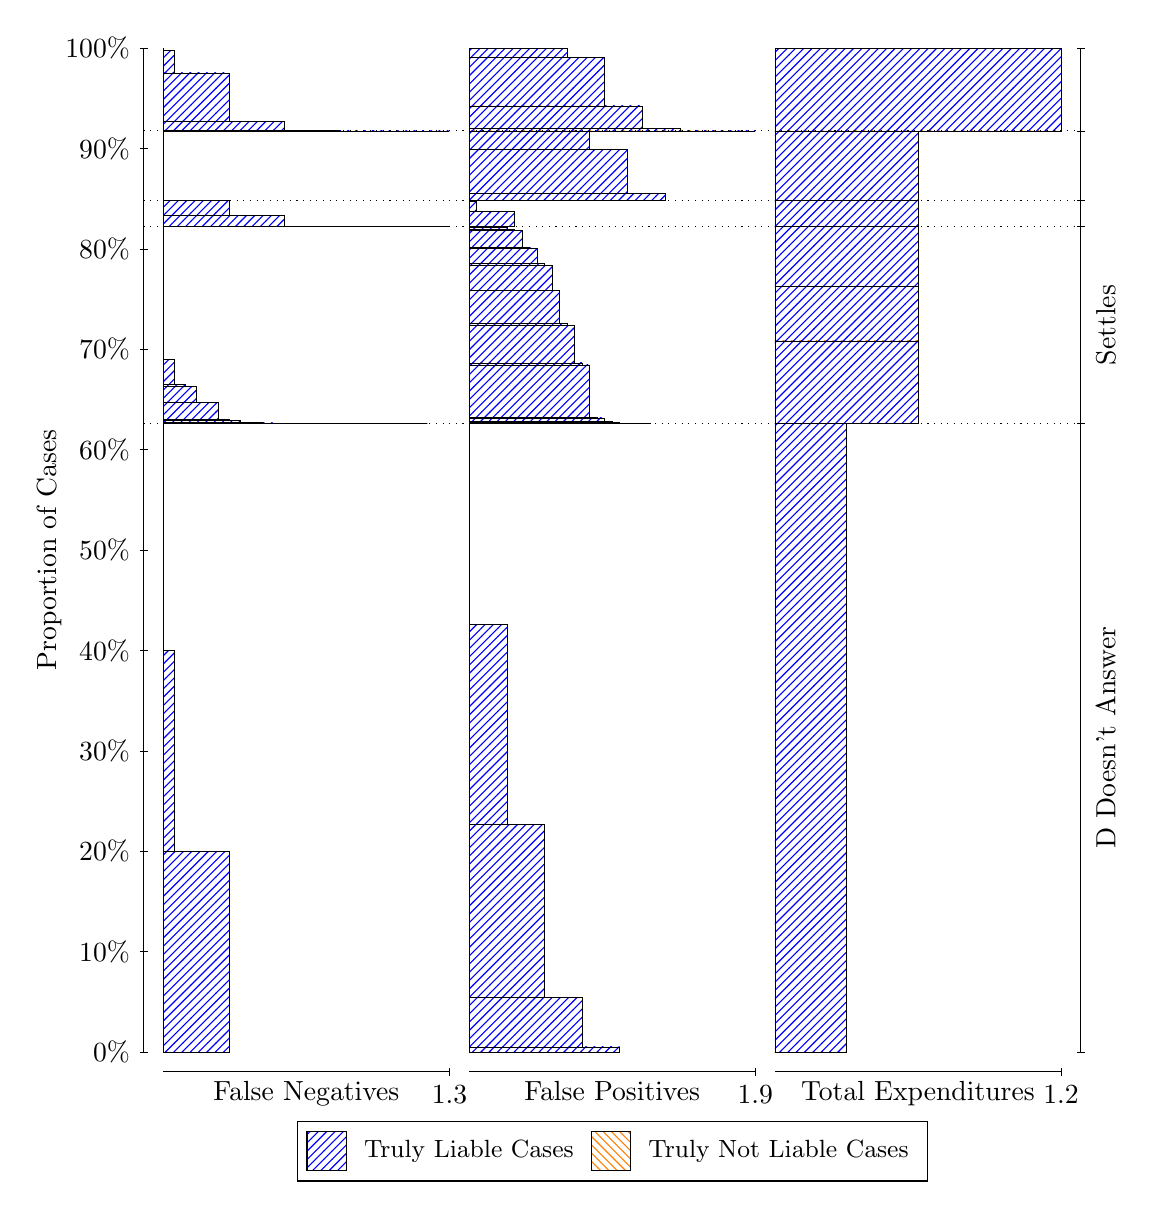
\begin{tikzpicture}
\draw[black, very thin] (1.5,1.75) -- (1.5,14.5);
\node[rotate=90, anchor=center] at (0.3, 8.125) {Proportion of Cases};
\draw[black, very thin] (1.45,1.75) -- (1.55,1.75);
\node[anchor=east] at (1.45, 1.75) {0\%};
\draw[black, very thin] (1.45,3.025) -- (1.55,3.025);
\node[anchor=east] at (1.45, 3.025) {10\%};
\draw[black, very thin] (1.45,4.3) -- (1.55,4.3);
\node[anchor=east] at (1.45, 4.3) {20\%};
\draw[black, very thin] (1.45,5.575) -- (1.55,5.575);
\node[anchor=east] at (1.45, 5.575) {30\%};
\draw[black, very thin] (1.45,6.85) -- (1.55,6.85);
\node[anchor=east] at (1.45, 6.85) {40\%};
\draw[black, very thin] (1.45,8.125) -- (1.55,8.125);
\node[anchor=east] at (1.45, 8.125) {50\%};
\draw[black, very thin] (1.45,9.4) -- (1.55,9.4);
\node[anchor=east] at (1.45, 9.4) {60\%};
\draw[black, very thin] (1.45,10.675) -- (1.55,10.675);
\node[anchor=east] at (1.45, 10.675) {70\%};
\draw[black, very thin] (1.45,11.95) -- (1.55,11.95);
\node[anchor=east] at (1.45, 11.95) {80\%};
\draw[black, very thin] (1.45,13.225) -- (1.55,13.225);
\node[anchor=east] at (1.45, 13.225) {90\%};
\draw[black, very thin] (1.45,14.5) -- (1.55,14.5);
\node[anchor=east] at (1.45, 14.5) {100\%};

\draw[black, very thin] (13.4,1.75) -- (13.4,14.5);
\draw[black, very thin] (13.35,1.75) -- (13.45,1.75);
\node[anchor=west] at (13.35, 1.75) {};
\draw[black, very thin] (13.35,9.7326) -- (13.45,9.7326);
\node[anchor=west] at (13.35, 9.7326) {};
\draw[black, very thin] (13.35,12.234) -- (13.45,12.234);
\node[anchor=west] at (13.35, 12.234) {};
\draw[black, very thin] (13.35,12.564) -- (13.45,12.564);
\node[anchor=west] at (13.35, 12.564) {};
\draw[black, very thin] (13.35,13.448) -- (13.45,13.448);
\node[anchor=west] at (13.35, 13.448) {};
\draw[black, very thin] (13.35,14.5) -- (13.45,14.5);
\node[anchor=west] at (13.35, 14.5) {};

\draw[black, very thin, pattern color=blue, pattern=north east lines] (1.75,1.75) rectangle (2.5885,4.2999);
\draw[black, very thin, pattern color=blue, pattern=north east lines] (1.75,4.2999) rectangle (1.8897,6.8469);
\draw[black, very thin, pattern color=orange, pattern=north west lines] (1.75,6.8469) rectangle (1.75,6.8469);
\draw[black, very thin, pattern color=blue, pattern=north east lines] (1.75,6.8469) rectangle (1.75,9.7326);
\draw[black, very thin, pattern color=blue, pattern=north east lines] (1.75,9.7326) rectangle (5.1038,9.7326);
\draw[black, very thin, pattern color=blue, pattern=north east lines] (1.75,9.7326) rectangle (4.8244,9.7326);
\draw[black, very thin, pattern color=blue, pattern=north east lines] (1.75,9.7326) rectangle (4.5449,9.7326);
\draw[black, very thin, pattern color=blue, pattern=north east lines] (1.75,9.7326) rectangle (4.4051,9.7326);
\draw[black, very thin, pattern color=blue, pattern=north east lines] (1.75,9.7326) rectangle (4.2654,9.7326);
\draw[black, very thin, pattern color=blue, pattern=north east lines] (1.75,9.7326) rectangle (4.2654,9.7326);
\draw[black, very thin, pattern color=blue, pattern=north east lines] (1.75,9.7326) rectangle (4.1256,9.7326);
\draw[black, very thin, pattern color=blue, pattern=north east lines] (1.75,9.7326) rectangle (3.9859,9.7326);
\draw[black, very thin, pattern color=blue, pattern=north east lines] (1.75,9.7326) rectangle (3.8462,9.7326);
\draw[black, very thin, pattern color=blue, pattern=north east lines] (1.75,9.7326) rectangle (3.7064,9.7328);
\draw[black, very thin, pattern color=blue, pattern=north east lines] (1.75,9.7328) rectangle (3.5667,9.7328);
\draw[black, very thin, pattern color=blue, pattern=north east lines] (1.75,9.7328) rectangle (3.5667,9.7328);
\draw[black, very thin, pattern color=blue, pattern=north east lines] (1.75,9.7328) rectangle (3.4269,9.7328);
\draw[black, very thin, pattern color=blue, pattern=north east lines] (1.75,9.7328) rectangle (3.4269,9.7336);
\draw[black, very thin, pattern color=blue, pattern=north east lines] (1.75,9.7336) rectangle (3.2872,9.7337);
\draw[black, very thin, pattern color=blue, pattern=north east lines] (1.75,9.7337) rectangle (3.1474,9.7406);
\draw[black, very thin, pattern color=blue, pattern=north east lines] (1.75,9.7406) rectangle (3.0077,9.7407);
\draw[black, very thin, pattern color=blue, pattern=north east lines] (1.75,9.7407) rectangle (3.0077,9.7433);
\draw[black, very thin, pattern color=blue, pattern=north east lines] (1.75,9.7433) rectangle (2.8679,9.7433);
\draw[black, very thin, pattern color=blue, pattern=north east lines] (1.75,9.7433) rectangle (2.8679,9.749);
\draw[black, very thin, pattern color=blue, pattern=north east lines] (1.75,9.749) rectangle (2.8679,9.749);
\draw[black, very thin, pattern color=blue, pattern=north east lines] (1.75,9.749) rectangle (2.7282,9.7491);
\draw[black, very thin, pattern color=blue, pattern=north east lines] (1.75,9.7491) rectangle (2.7282,9.7718);
\draw[black, very thin, pattern color=blue, pattern=north east lines] (1.75,9.7718) rectangle (2.5885,9.7847);
\draw[black, very thin, pattern color=blue, pattern=north east lines] (1.75,9.7847) rectangle (2.4487,10.002);
\draw[black, very thin, pattern color=blue, pattern=north east lines] (1.75,10.002) rectangle (2.309,10.003);
\draw[black, very thin, pattern color=blue, pattern=north east lines] (1.75,10.003) rectangle (2.309,10.004);
\draw[black, very thin, pattern color=blue, pattern=north east lines] (1.75,10.004) rectangle (2.1692,10.005);
\draw[black, very thin, pattern color=blue, pattern=north east lines] (1.75,10.005) rectangle (2.1692,10.198);
\draw[black, very thin, pattern color=blue, pattern=north east lines] (1.75,10.198) rectangle (2.1692,10.198);
\draw[black, very thin, pattern color=blue, pattern=north east lines] (1.75,10.198) rectangle (2.0295,10.202);
\draw[black, very thin, pattern color=blue, pattern=north east lines] (1.75,10.202) rectangle (2.0295,10.229);
\draw[black, very thin, pattern color=blue, pattern=north east lines] (1.75,10.229) rectangle (1.8897,10.547);
\draw[black, very thin, pattern color=orange, pattern=north west lines] (1.75,10.547) rectangle (1.75,10.547);
\draw[black, very thin, pattern color=blue, pattern=north east lines] (1.75,10.547) rectangle (1.75,12.234);
\draw[black, very thin, pattern color=blue, pattern=north east lines] (1.75,12.234) rectangle (5.3833,12.234);
\draw[black, very thin, pattern color=blue, pattern=north east lines] (1.75,12.234) rectangle (4.6846,12.234);
\draw[black, very thin, pattern color=blue, pattern=north east lines] (1.75,12.234) rectangle (3.9859,12.239);
\draw[black, very thin, pattern color=blue, pattern=north east lines] (1.75,12.239) rectangle (3.2872,12.37);
\draw[black, very thin, pattern color=blue, pattern=north east lines] (1.75,12.37) rectangle (2.5885,12.564);
\draw[black, very thin, pattern color=orange, pattern=north west lines] (1.75,12.564) rectangle (1.75,12.564);
\draw[black, very thin, pattern color=blue, pattern=north east lines] (1.75,12.564) rectangle (2.5885,12.564);
\draw[black, very thin, pattern color=blue, pattern=north east lines] (1.75,12.564) rectangle (1.8897,12.566);
\draw[black, very thin, pattern color=orange, pattern=north west lines] (1.75,12.566) rectangle (1.75,12.566);
\draw[black, very thin, pattern color=blue, pattern=north east lines] (1.75,12.566) rectangle (1.75,13.448);
\draw[black, very thin, pattern color=blue, pattern=north east lines] (1.75,13.448) rectangle (5.3833,13.448);
\draw[black, very thin, pattern color=blue, pattern=north east lines] (1.75,13.448) rectangle (4.6846,13.448);
\draw[black, very thin, pattern color=blue, pattern=north east lines] (1.75,13.448) rectangle (3.9859,13.45);
\draw[black, very thin, pattern color=blue, pattern=north east lines] (1.75,13.45) rectangle (3.2872,13.564);
\draw[black, very thin, pattern color=blue, pattern=north east lines] (1.75,13.564) rectangle (2.5885,13.564);
\draw[black, very thin, pattern color=blue, pattern=north east lines] (1.75,13.564) rectangle (2.5885,14.184);
\draw[black, very thin, pattern color=blue, pattern=north east lines] (1.75,14.184) rectangle (1.8897,14.184);
\draw[black, very thin, pattern color=blue, pattern=north east lines] (1.75,14.184) rectangle (1.8897,14.472);
\draw[black, very thin, pattern color=orange, pattern=north west lines] (1.75,14.472) rectangle (1.75,14.472);
\draw[black, very thin, pattern color=blue, pattern=north east lines] (1.75,14.472) rectangle (1.75,14.5);
\draw[black, very thin, pattern color=orange, pattern=north west lines] (5.6333,1.75) rectangle (7.5456,1.75);
\draw[black, very thin, pattern color=blue, pattern=north east lines] (5.6333,1.75) rectangle (7.5456,1.8143);
\draw[black, very thin, pattern color=blue, pattern=north east lines] (5.6333,1.8143) rectangle (7.0675,2.4396);
\draw[black, very thin, pattern color=blue, pattern=north east lines] (5.6333,2.4396) rectangle (6.5895,4.6357);
\draw[black, very thin, pattern color=blue, pattern=north east lines] (5.6333,4.6357) rectangle (6.1114,7.1827);
\draw[black, very thin, pattern color=blue, pattern=north east lines] (5.6333,7.1827) rectangle (5.6333,9.7326);
\draw[black, very thin, pattern color=orange, pattern=north west lines] (5.6333,9.7326) rectangle (7.9281,9.7326);
\draw[black, very thin, pattern color=blue, pattern=north east lines] (5.6333,9.7326) rectangle (7.9281,9.7331);
\draw[black, very thin, pattern color=orange, pattern=north west lines] (5.6333,9.7331) rectangle (7.7368,9.7331);
\draw[black, very thin, pattern color=blue, pattern=north east lines] (5.6333,9.7331) rectangle (7.7368,9.734);
\draw[black, very thin, pattern color=orange, pattern=north west lines] (5.6333,9.734) rectangle (7.5456,9.734);
\draw[black, very thin, pattern color=blue, pattern=north east lines] (5.6333,9.734) rectangle (7.5456,9.7465);
\draw[black, very thin, pattern color=blue, pattern=north east lines] (5.6333,9.7465) rectangle (7.45,9.7546);
\draw[black, very thin, pattern color=orange, pattern=north west lines] (5.6333,9.7546) rectangle (7.3544,9.7546);
\draw[black, very thin, pattern color=blue, pattern=north east lines] (5.6333,9.7546) rectangle (7.3544,9.8025);
\draw[black, very thin, pattern color=blue, pattern=north east lines] (5.6333,9.8025) rectangle (7.2588,9.8096);
\draw[black, very thin, pattern color=orange, pattern=north west lines] (5.6333,9.8096) rectangle (7.1632,9.8096);
\draw[black, very thin, pattern color=blue, pattern=north east lines] (5.6333,9.8096) rectangle (7.1632,10.475);
\draw[black, very thin, pattern color=blue, pattern=north east lines] (5.6333,10.475) rectangle (7.0675,10.5);
\draw[black, very thin, pattern color=orange, pattern=north west lines] (5.6333,10.5) rectangle (6.9719,10.5);
\draw[black, very thin, pattern color=blue, pattern=north east lines] (5.6333,10.5) rectangle (6.9719,10.974);
\draw[black, very thin, pattern color=blue, pattern=north east lines] (5.6333,10.974) rectangle (6.8763,11.005);
\draw[black, very thin, pattern color=blue, pattern=north east lines] (5.6333,11.005) rectangle (6.7807,11.007);
\draw[black, very thin, pattern color=orange, pattern=north west lines] (5.6333,11.007) rectangle (6.7807,11.007);
\draw[black, very thin, pattern color=blue, pattern=north east lines] (5.6333,11.007) rectangle (6.7807,11.42);
\draw[black, very thin, pattern color=blue, pattern=north east lines] (5.6333,11.42) rectangle (6.6851,11.738);
\draw[black, very thin, pattern color=orange, pattern=north west lines] (5.6333,11.738) rectangle (6.5895,11.738);
\draw[black, very thin, pattern color=blue, pattern=north east lines] (5.6333,11.738) rectangle (6.5895,11.769);
\draw[black, very thin, pattern color=blue, pattern=north east lines] (5.6333,11.769) rectangle (6.4939,11.963);
\draw[black, very thin, pattern color=orange, pattern=north west lines] (5.6333,11.963) rectangle (6.3982,11.963);
\draw[black, very thin, pattern color=blue, pattern=north east lines] (5.6333,11.963) rectangle (6.3982,11.964);
\draw[black, very thin, pattern color=blue, pattern=north east lines] (5.6333,11.964) rectangle (6.3982,11.965);
\draw[black, very thin, pattern color=blue, pattern=north east lines] (5.6333,11.965) rectangle (6.3026,11.965);
\draw[black, very thin, pattern color=blue, pattern=north east lines] (5.6333,11.965) rectangle (6.3026,12.182);
\draw[black, very thin, pattern color=blue, pattern=north east lines] (5.6333,12.182) rectangle (6.207,12.195);
\draw[black, very thin, pattern color=blue, pattern=north east lines] (5.6333,12.195) rectangle (6.1114,12.218);
\draw[black, very thin, pattern color=blue, pattern=north east lines] (5.6333,12.218) rectangle (6.0158,12.224);
\draw[black, very thin, pattern color=blue, pattern=north east lines] (5.6333,12.224) rectangle (5.9202,12.226);
\draw[black, very thin, pattern color=blue, pattern=north east lines] (5.6333,12.226) rectangle (5.9202,12.226);
\draw[black, very thin, pattern color=blue, pattern=north east lines] (5.6333,12.226) rectangle (5.8246,12.226);
\draw[black, very thin, pattern color=blue, pattern=north east lines] (5.6333,12.226) rectangle (5.8246,12.233);
\draw[black, very thin, pattern color=blue, pattern=north east lines] (5.6333,12.233) rectangle (5.7289,12.233);
\draw[black, very thin, pattern color=blue, pattern=north east lines] (5.6333,12.233) rectangle (5.6333,12.234);
\draw[black, very thin, pattern color=orange, pattern=north west lines] (5.6333,12.234) rectangle (6.207,12.234);
\draw[black, very thin, pattern color=blue, pattern=north east lines] (5.6333,12.234) rectangle (6.207,12.428);
\draw[black, very thin, pattern color=blue, pattern=north east lines] (5.6333,12.428) rectangle (5.7289,12.559);
\draw[black, very thin, pattern color=blue, pattern=north east lines] (5.6333,12.559) rectangle (5.6333,12.564);
\draw[black, very thin, pattern color=orange, pattern=north west lines] (5.6333,12.564) rectangle (8.1193,12.564);
\draw[black, very thin, pattern color=blue, pattern=north east lines] (5.6333,12.564) rectangle (8.1193,12.656);
\draw[black, very thin, pattern color=blue, pattern=north east lines] (5.6333,12.656) rectangle (7.6412,13.217);
\draw[black, very thin, pattern color=blue, pattern=north east lines] (5.6333,13.217) rectangle (7.1632,13.446);
\draw[black, very thin, pattern color=blue, pattern=north east lines] (5.6333,13.446) rectangle (6.6851,13.448);
\draw[black, very thin, pattern color=blue, pattern=north east lines] (5.6333,13.448) rectangle (6.207,13.448);
\draw[black, very thin, pattern color=orange, pattern=north west lines] (5.6333,13.448) rectangle (9.2667,13.448);
\draw[black, very thin, pattern color=blue, pattern=north east lines] (5.6333,13.448) rectangle (9.2667,13.448);
\draw[black, very thin, pattern color=orange, pattern=north west lines] (5.6333,13.448) rectangle (8.7886,13.448);
\draw[black, very thin, pattern color=blue, pattern=north east lines] (5.6333,13.448) rectangle (8.7886,13.449);
\draw[black, very thin, pattern color=orange, pattern=north west lines] (5.6333,13.449) rectangle (8.3105,13.449);
\draw[black, very thin, pattern color=blue, pattern=north east lines] (5.6333,13.449) rectangle (8.3105,13.477);
\draw[black, very thin, pattern color=orange, pattern=north west lines] (5.6333,13.477) rectangle (7.8325,13.477);
\draw[black, very thin, pattern color=blue, pattern=north east lines] (5.6333,13.477) rectangle (7.8325,13.764);
\draw[black, very thin, pattern color=orange, pattern=north west lines] (5.6333,13.764) rectangle (7.3544,13.764);
\draw[black, very thin, pattern color=blue, pattern=north east lines] (5.6333,13.764) rectangle (7.3544,14.384);
\draw[black, very thin, pattern color=blue, pattern=north east lines] (5.6333,14.384) rectangle (6.8763,14.498);
\draw[black, very thin, pattern color=blue, pattern=north east lines] (5.6333,14.498) rectangle (6.3982,14.5);
\draw[black, very thin, pattern color=blue, pattern=north east lines] (5.6333,14.5) rectangle (5.9202,14.5);
\draw[black, very thin, pattern color=blue, pattern=north east lines] (5.6333,14.5) rectangle (5.6333,14.5);
\draw[black, very thin, pattern color=orange, pattern=north west lines] (9.5167,1.75) rectangle (10.425,1.75);
\draw[black, very thin, pattern color=blue, pattern=north east lines] (9.5167,1.75) rectangle (10.425,9.7326);
\draw[black, very thin, pattern color=orange, pattern=north west lines] (9.5167,9.7326) rectangle (11.333,9.7326);
\draw[black, very thin, pattern color=blue, pattern=north east lines] (9.5167,9.7326) rectangle (11.333,10.78);
\draw[black, very thin, pattern color=orange, pattern=north west lines] (9.5167,10.78) rectangle (11.333,10.78);
\draw[black, very thin, pattern color=blue, pattern=north east lines] (9.5167,10.78) rectangle (11.333,11.476);
\draw[black, very thin, pattern color=orange, pattern=north west lines] (9.5167,11.476) rectangle (11.333,11.476);
\draw[black, very thin, pattern color=blue, pattern=north east lines] (9.5167,11.476) rectangle (11.333,12.234);
\draw[black, very thin, pattern color=orange, pattern=north west lines] (9.5167,12.234) rectangle (11.333,12.234);
\draw[black, very thin, pattern color=blue, pattern=north east lines] (9.5167,12.234) rectangle (11.333,12.564);
\draw[black, very thin, pattern color=orange, pattern=north west lines] (9.5167,12.564) rectangle (11.333,12.564);
\draw[black, very thin, pattern color=blue, pattern=north east lines] (9.5167,12.564) rectangle (11.333,13.448);
\draw[black, very thin, pattern color=orange, pattern=north west lines] (9.5167,13.448) rectangle (13.15,13.448);
\draw[black, very thin, pattern color=blue, pattern=north east lines] (9.5167,13.448) rectangle (13.15,14.5);
\draw[black, dotted] (1.5,9.7326) -- (13.4,9.7326);
\draw[black, dotted] (1.5,12.234) -- (13.4,12.234);
\draw[black, dotted] (1.5,12.564) -- (13.4,12.564);
\draw[black, dotted] (1.5,13.448) -- (13.4,13.448);
\draw[black, very thin] (1.75,1.5) -- (5.3833,1.5);
\node[anchor=north] at (3.5667, 1.5) {False Negatives};
\draw[black, very thin] (5.3833,1.45) -- (5.3833,1.55);
\node[anchor=north] at (5.3833, 1.45) {1.3};

\draw[black, very thin] (5.6333,1.5) -- (9.2667,1.5);
\node[anchor=north] at (7.45, 1.5) {False Positives};
\draw[black, very thin] (9.2667,1.45) -- (9.2667,1.55);
\node[anchor=north] at (9.2667, 1.45) {1.9};

\draw[black, very thin] (9.5167,1.5) -- (13.15,1.5);
\node[anchor=north] at (11.333, 1.5) {Total Expenditures};
\draw[black, very thin] (13.15,1.45) -- (13.15,1.55);
\node[anchor=north] at (13.15, 1.45) {1.2};

\node[black, centered, rotate=90] at (13.72, 5.7413) {D Doesn't Answer};
\node[black, centered, rotate=90] at (13.72, 10.983) {Settles};




\draw (7.449999999999999,1.5) node[draw=none] (baseCoordinate) {};
\begin{scope}[align=center]
        \matrix[scale=0.5, draw=black, below=0.5cm of baseCoordinate, nodes={draw}, column sep=0.1cm]{
            \node[rectangle, draw, minimum width=0.5cm, minimum height=0.5cm, pattern=north east lines, pattern color=blue] {}; &
            \node[draw=none, font=\small] (B) {Truly Liable Cases}; &
            \node[rectangle, draw, minimum width=0.5cm, minimum height=0.5cm, pattern=north west lines, pattern color=orange] {}; &
            \node[draw=none, font=\small] (B) {Truly Not Liable Cases}; \\
            };
\end{scope}

\end{tikzpicture}
\end{document}